\section{L'interconnexion avec les autres sites}
\subsection{Mise en place de l’interconnexion entre AS}

L'un des objectifs majeurs de ce projet était de réaliser une interconnexion globale avec les Systèmes Autonomes (AS) des autres groupes de la classe. Pour y parvenir, nous avons déployé le protocole eBGP, indispensable pour l'échange dynamique de routes inter-domaines.\\

Concrètement, nous avons configuré notre routeur de bordure R4 afin d'établir des sessions de peering directes avec les AS voisins (AS 11, 12 et 13). Pour optimiser ces échanges, nous avons mis en place une agrégation de routes permettant d'annoncer un préfixe unique en /20 (120.0.0.0/20), sécurisé par une route statique vers l'interface virtuelle Null0. De plus, afin que notre réseau interne profite de ces routes externes, nous avons configuré la redistribution des routes BGP au sein de notre protocole de routage interne OSPF. La réussite de cette architecture a été validée par la convergence globale des tables et l'établissement stable des voisinages.\\

\begin{figure}[!ht]
    \centering
    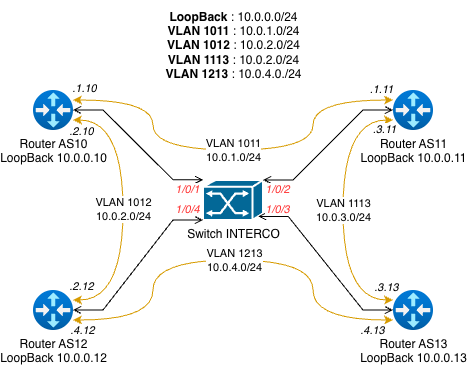
\includegraphics[width=1\linewidth]{image/schema_archi/Schema Reseau Interconnexion.png}
    \caption{Schéma technique du réseau d'interconnexion}
    \label{fig:schema_technique_reseau_interco}
\end{figure}

Le succès des interconnexions a été démontré et validé lors de la présentation orale du projet.